% =========================================================
% SECTION: SCHEDULING
% =========================================================

\section{CPU Scheduling}

% ---------------------------------------------------------
\begin{frame}{From Mechanisms to Scheduling}

\begin{itemize}
    \item We now understand the low-level mechanisms for running processes:
    \begin{itemize}
        \item timer interrupts;
        \item context switching;
        \item switching between processes.
    \end{itemize}

    \item The next question concerns \textbf{policy}:
    \begin{itemize}
        \item Which process should run?
        \item When should it run?
        \item For how long?
    \end{itemize}
\end{itemize}

\begin{block}{The Crux}
How should we develop a basic framework for thinking about
\textbf{scheduling policies}?
\end{block}

\end{frame}

% ---------------------------------------------------------
\begin{frame}{Workload Assumptions}

To develop basic scheduling policies, we initially assume:

\begin{enumerate}
    \item Each job runs for the same amount of time.
    \item All jobs arrive at the same time.
    \item Once started, each job runs to completion.
    \item Jobs use only the CPU and perform no I/O.
    \item The run-time of each job is known.
\end{enumerate}

\medskip

These assumptions are intentionally unrealistic and will be
\textbf{relaxed progressively}.

\end{frame}

% ---------------------------------------------------------
\begin{frame}{Scheduling Metrics}

The main performance metric initially considered is
\textbf{turnaround time}:

\[
T_{\text{turnaround}}
=
T_{\text{completion}}
-
T_{\text{arrival}}
\]

With all jobs arriving at \(t=0\):

\[
T_{\text{turnaround}} = T_{\text{completion}}
\]

\begin{block}{Performance vs. Fairness}
Scheduling policies may improve performance at the cost of fairness,
or improve fairness at the cost of performance.
\end{block}

\end{frame}

% ---------------------------------------------------------
\begin{frame}{First In, First Out (FIFO)}

\begin{columns}[T]

\column{0.43\textwidth}

\begin{itemize}
    \item Also called \textbf{First Come, First Served (FCFS)}.
    \item Simple and easy to implement.
    \item Jobs execute in arrival order.
\end{itemize}

\medskip

Example:

\[
A = B = C = 10
\]

\[
\overline{T}_{turnaround}
=
\frac{10+20+30}{3}
=
20
\]

\column{0.55\textwidth}
\begin{figure}
    \centering
    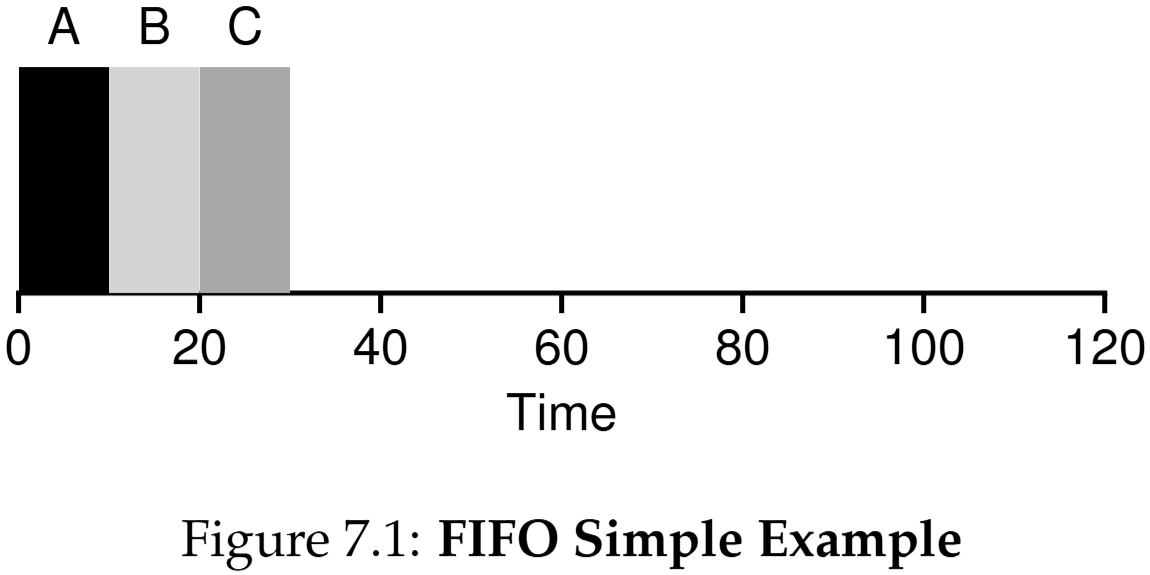
\includegraphics[width=1.1\linewidth]{figs/chapter-7/figure-7.1.png}
    \caption*{Source: chapter page 3.}
    \label{fig:figure-7.1}
\end{figure}
\end{columns}

\end{frame}

% ---------------------------------------------------------
\begin{frame}{The Convoy Effect}

Relax assumption 1: jobs may have \textbf{different lengths}.

\begin{columns}[T]

\column{0.43\textwidth}

Example:

\[
A=100,\qquad B=C=10
\]

Under FIFO:

\[
\overline{T}_{turnaround}
=
\frac{100+110+120}{3}
=
110
\]

\begin{block}{Convoy Effect}
Short jobs wait behind a long-running job.
\end{block}

\column{0.55\textwidth}
\begin{figure}
    \centering
    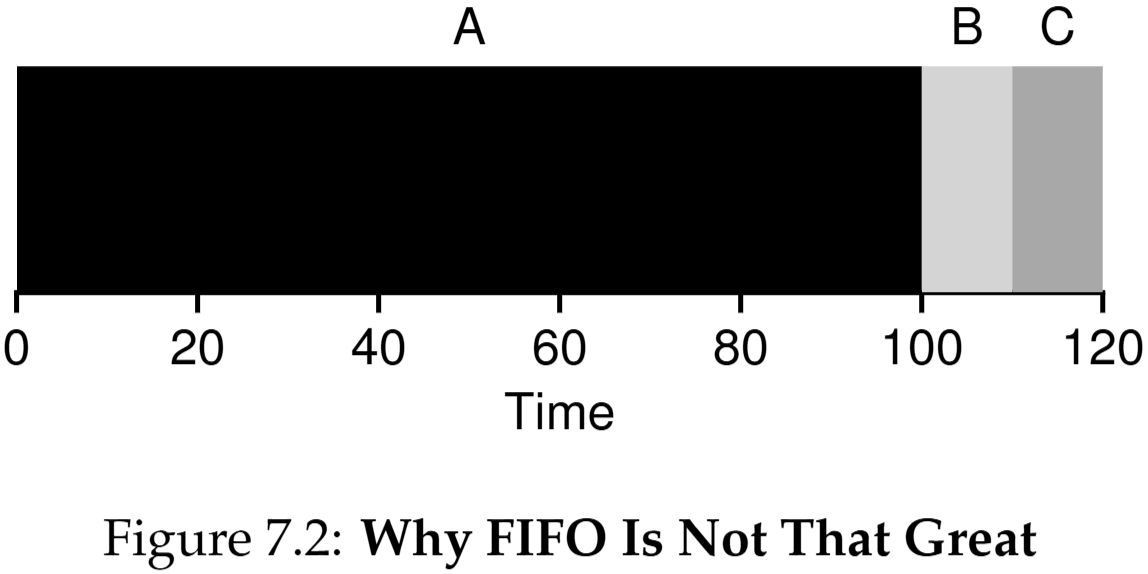
\includegraphics[width=1.1\linewidth]{figs/chapter-7/figure-7.2.png}
    \caption*{Source: chapter page 3.}
    \label{fig:figure-7.2}
\end{figure}
\end{columns}

\end{frame}

% ---------------------------------------------------------
\begin{frame}{Shortest Job First (SJF)}

\begin{columns}[T]

\column{0.43\textwidth}

\textbf{Shortest Job First (SJF)} executes jobs in increasing order
of run time.

\medskip

For:

\[
A=100,\qquad B=C=10
\]

SJF executes:

\[
B \rightarrow C \rightarrow A
\]

and obtains:

\[
\overline{T}_{turnaround}
=
\frac{10+20+120}{3}
=
50
\]

\column{0.55\textwidth}
\begin{figure}
    \centering
    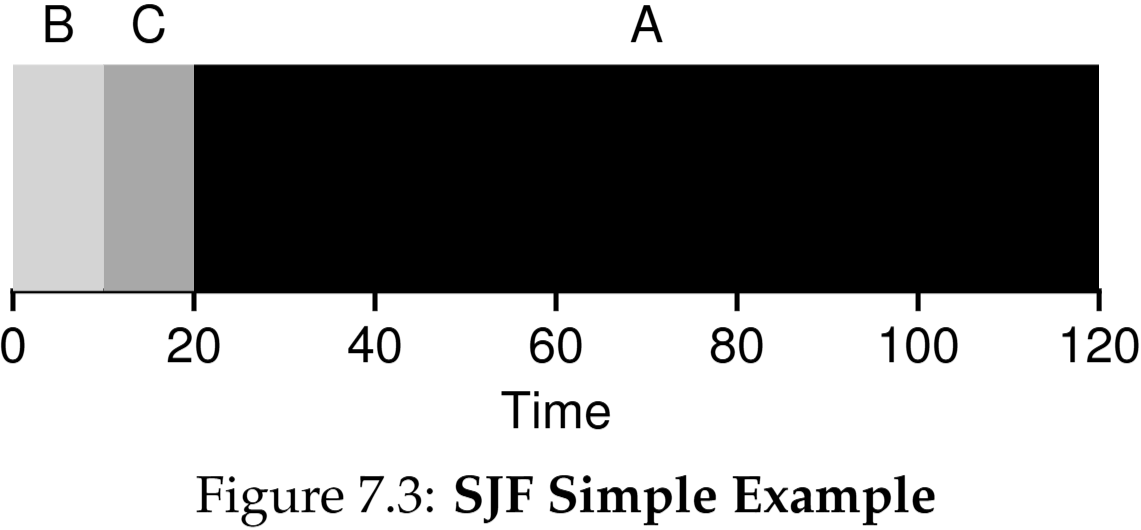
\includegraphics[width=1.1\linewidth]{figs/chapter-7/figure-7.3.png}
    \caption*{Source: chapter page 4.}
    \label{fig:figure-7.3}
\end{figure}
\end{columns}

\end{frame}

% ---------------------------------------------------------
\begin{frame}{SJF and Late Arrivals}

Now relax assumption 2: jobs may arrive at
\textbf{different times}.

\begin{columns}[T]

\column{0.43\textwidth}

Example:

\begin{itemize}
    \item \(A\) arrives at \(t=0\), requiring 100 s.
    \item \(B\) and \(C\) arrive at \(t=10\), requiring 10 s each.
\end{itemize}

Because SJF is non-preemptive, \(B\) and \(C\) must still wait for
\(A\).

\[
\overline{T}_{turnaround}=103.33
\]

\column{0.55\textwidth}
\begin{figure}
    \centering
    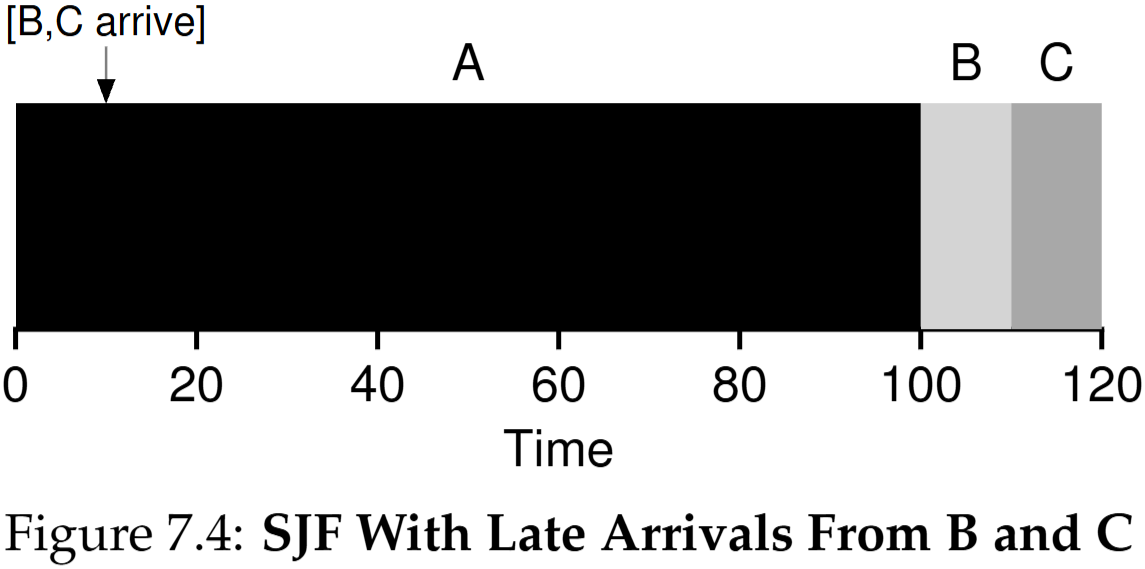
\includegraphics[width=1.1\linewidth]{figs/chapter-7/figure-7.4.png}
    \caption*{Source: chapter page 5.}
    \label{fig:figure-7.4}
\end{figure}
\end{columns}

\end{frame}

% ---------------------------------------------------------
\begin{frame}{Shortest Time-to-Completion First (STCF)}

Relax assumption 3: a running job may be
\textbf{preempted}.

\begin{columns}[T]

\column{0.43\textwidth}

\textbf{STCF} is the preemptive version of SJF.

\begin{itemize}
    \item When a new job arrives, compare the remaining execution times.
    \item Run the job with the least time remaining.
    \item A running process may therefore be preempted.
\end{itemize}

For the previous example:

\[
\overline{T}_{turnaround}=50
\]

\column{0.55\textwidth}
\begin{figure}
    \centering
    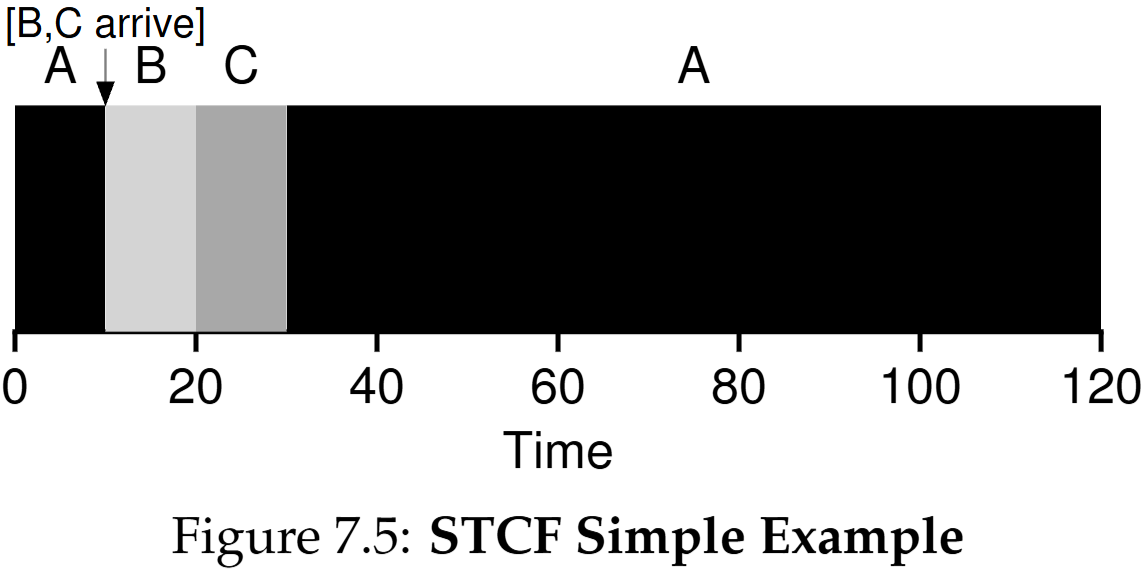
\includegraphics[width=1.1\linewidth]{figs/chapter-7/figure-7.5.png}
    \caption*{Source: chapter page 6.}
    \label{fig:figure-7.5}
\end{figure}
\end{columns}

\end{frame}

% ---------------------------------------------------------
\begin{frame}{A New Metric: Response Time}

Interactive systems require another metric:
\textbf{response time}.

\[
T_{\text{response}}
=
T_{\text{firstrun}}
-
T_{\text{arrival}}
\]

\begin{itemize}
    \item Turnaround time focuses on \textbf{completion}.
    \item Response time focuses on how quickly a job
          \textbf{starts receiving CPU time}.
    \item SJF/STCF may provide excellent turnaround time but poor
          interactive response.
\end{itemize}

\end{frame}

% ---------------------------------------------------------
\begin{frame}{SJF vs. Round Robin}

\begin{columns}[T]

\column{0.49\textwidth}

\centering

\textbf{SJF}

\vspace{0.2cm}

\begin{figure}
    \centering
    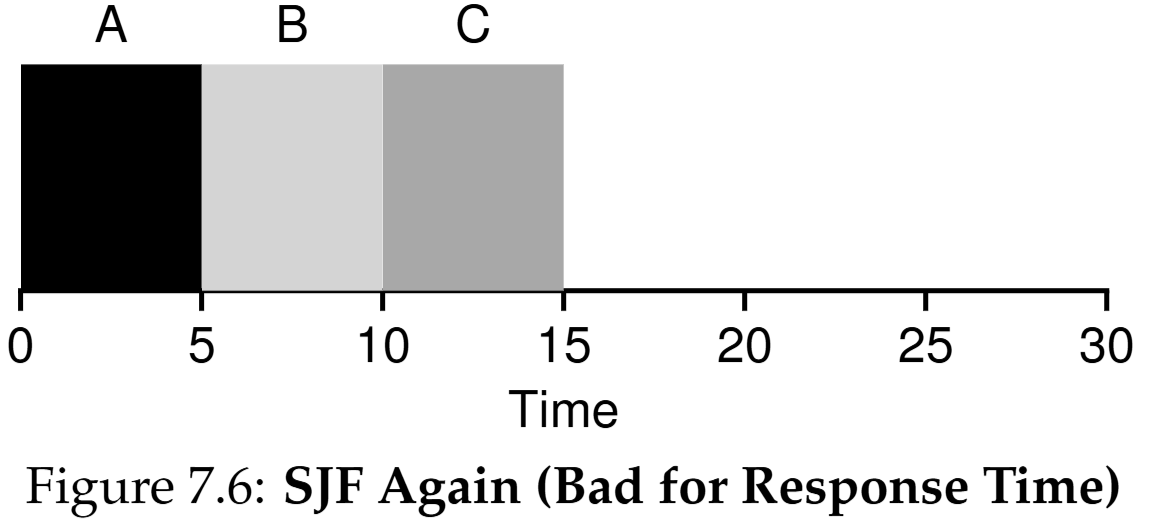
\includegraphics[width=1.1\linewidth]{figs/chapter-7/figure-7.6.png}
    \caption*{Source: chapter page 7.}
    \label{fig:figure-7.6}
\end{figure}

\[
\overline{T}_{response}
=
\frac{0+5+10}{3}=5
\]

\column{0.49\textwidth}

\centering

\textbf{Round Robin}

\vspace{0.2cm}

\begin{figure}
    \centering
    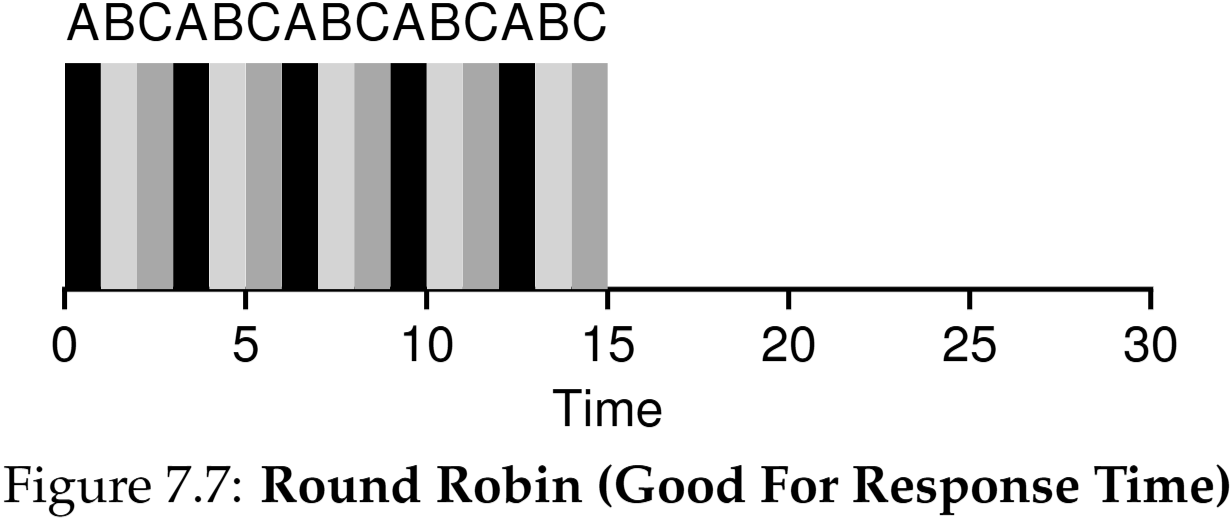
\includegraphics[width=1.1\linewidth]{figs/chapter-7/figure-7.7.png}
    \caption*{Source: chapter page 7.}
    \label{fig:figure-7.7}
\end{figure}

\[
\overline{T}_{response}
=
\frac{0+1+2}{3}=1
\]

\end{columns}

\end{frame}

% ---------------------------------------------------------
\begin{frame}{Round Robin (RR)}

Round Robin introduces \textbf{time slicing}.

\begin{itemize}
    \item Each job runs for a fixed \textbf{time slice} or
          \textbf{scheduling quantum}.
    \item After the quantum expires, the scheduler switches to the
          next job in the run queue.
    \item The process repeats until all jobs finish.
\end{itemize}

\begin{block}{Time-Slice Trade-off}
A shorter time slice improves response time, but increases the
relative cost of context switching.
\end{block}

\begin{itemize}
    \item Example: 10 ms quantum + 1 ms context switch
          \(\Rightarrow\) roughly 10\% switching overhead.
    \item Increasing the quantum amortizes this fixed cost.
\end{itemize}

\end{frame}

% ---------------------------------------------------------
\begin{frame}{Turnaround Time vs. Response Time}

The scheduling policies studied so far optimize different goals.

\begin{table}
\centering
\small

\begin{tabular}{lcc}
\hline
\textbf{Policy} &
\textbf{Turnaround} &
\textbf{Response} \\
\hline
FIFO      & workload-dependent & poor with convoy effect \\
SJF       & very good          & potentially poor \\
STCF      & very good          & potentially poor \\
RR        & poor               & very good \\
\hline
\end{tabular}

\end{table}

\begin{block}{Fundamental Trade-off}
Policies that divide CPU time fairly among active processes tend to
improve response time, but usually increase turnaround time.
\end{block}

\end{frame}

% ---------------------------------------------------------
\begin{frame}{Incorporating I/O}

Relax assumption 4: processes may perform \textbf{I/O}.

\begin{itemize}
    \item A process issuing I/O becomes blocked.
    \item The scheduler can run another process while the I/O proceeds.
    \item When the I/O completes, the blocked process becomes ready again.
\end{itemize}

\medskip

Example:

\begin{itemize}
    \item Job A: five 10-ms CPU bursts separated by I/O.
    \item Job B: one continuous 50-ms CPU burst.
\end{itemize}

\end{frame}

% ---------------------------------------------------------
\begin{frame}{Overlapping CPU and I/O}

\begin{columns}[T]

\column{0.49\textwidth}

\centering

\textbf{Poor Resource Use}

\vspace{0.2cm}

\begin{figure}
    \centering
    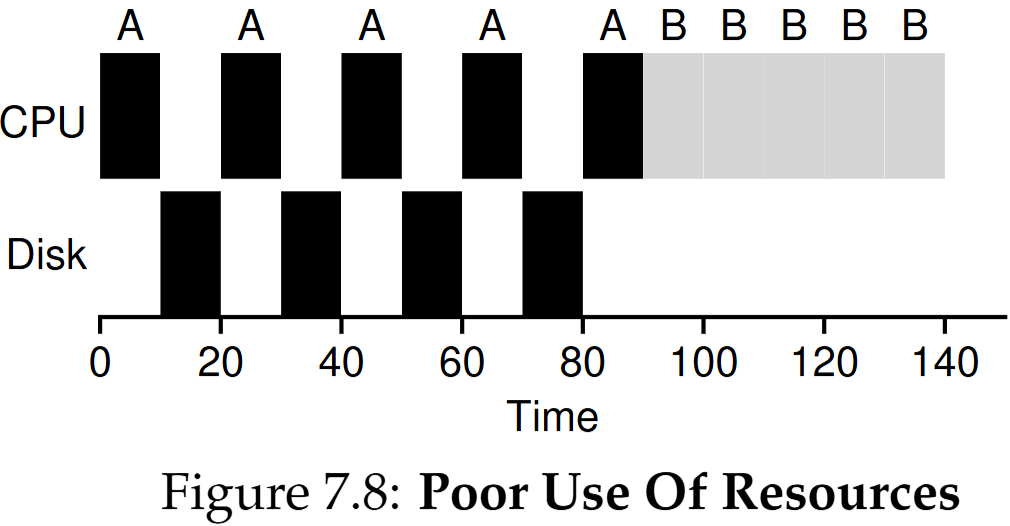
\includegraphics[width=1.1\linewidth]{figs/chapter-7/figure-7.8.png}
    \caption*{Source: chapter page 10.}
    \label{fig:figure-7.8}
\end{figure}

\column{0.49\textwidth}

\centering

\textbf{CPU/I/O Overlap}

\vspace{0.2cm}

\begin{figure}
    \centering
    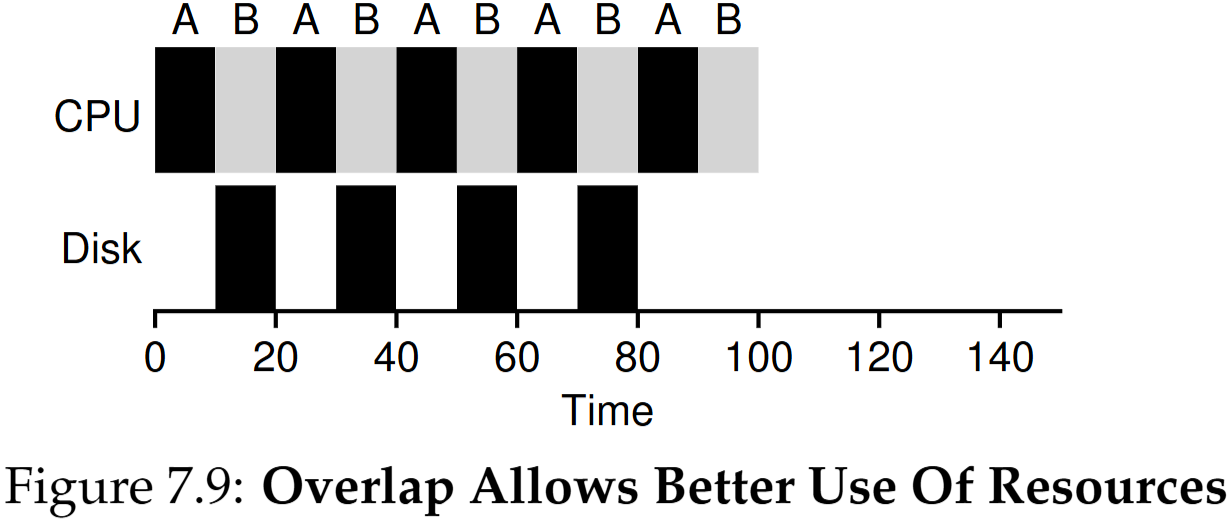
\includegraphics[width=1.1\linewidth]{figs/chapter-7/figure-7.9.png}
    \caption*{Source: chapter page 10.}
    \label{fig:figure-7.9}
\end{figure}

\end{columns}

\vspace{0.3cm}

\begin{block}{Key Idea}
Treating each CPU burst as a separate job enables CPU execution to
overlap with another process's I/O, improving system utilization.
\end{block}

\end{frame}

% ---------------------------------------------------------
\begin{frame}{No More Oracle}

One assumption still remains:

\begin{center}
\textbf{The scheduler knows the run-time of each job.}
\end{center}

In a general-purpose operating system, this information is normally
\textbf{not known in advance}.

\medskip

The remaining challenge is therefore:

\begin{itemize}
    \item obtain SJF/STCF-like turnaround behavior;
    \item preserve good response time;
    \item operate without knowing future job lengths.
\end{itemize}

\begin{block}{Next Step}
Use the \textbf{recent past to predict the future}:
the Multi-Level Feedback Queue (MLFQ).
\end{block}

\end{frame}

% ---------------------------------------------------------
\begin{frame}{CPU Scheduling: Summary}

\begin{itemize}
    \item Scheduling policy determines \textbf{which process runs}.
    \item \textbf{FIFO} is simple but may suffer from the convoy effect.
    \item \textbf{SJF/STCF} optimize turnaround time.
    \item \textbf{Round Robin} improves response time through time slicing.
    \item Response time and turnaround time represent an inherent
          scheduling trade-off.
    \item CPU and I/O can be overlapped to improve utilization.
    \item Real systems must schedule without knowing future job lengths.
\end{itemize}

\medskip

\begin{center}
\textbf{Next: Multi-Level Feedback Queue (MLFQ)}
\end{center}

\end{frame}